\documentclass{article}

\usepackage{tikz}
\usepackage{verbatim}
\usepackage{amssymb}

\begin{document}
\pagestyle{empty}
\def\layersep{2.5cm} % Seems like this defines a variable (bit like in less)

\begin{comment}
    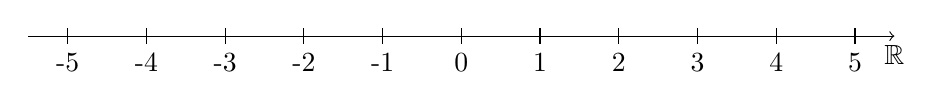
\begin{tikzpicture}
	\draw[->](-5.5, 0) -- (5.5, 0) node [below] { $\mathbb{R}$ };
	\foreach \x in {-5,...,5}
		\draw (\x, 0.1) -- (\x, -0.1) node [below] { \x };
    \end{tikzpicture}

    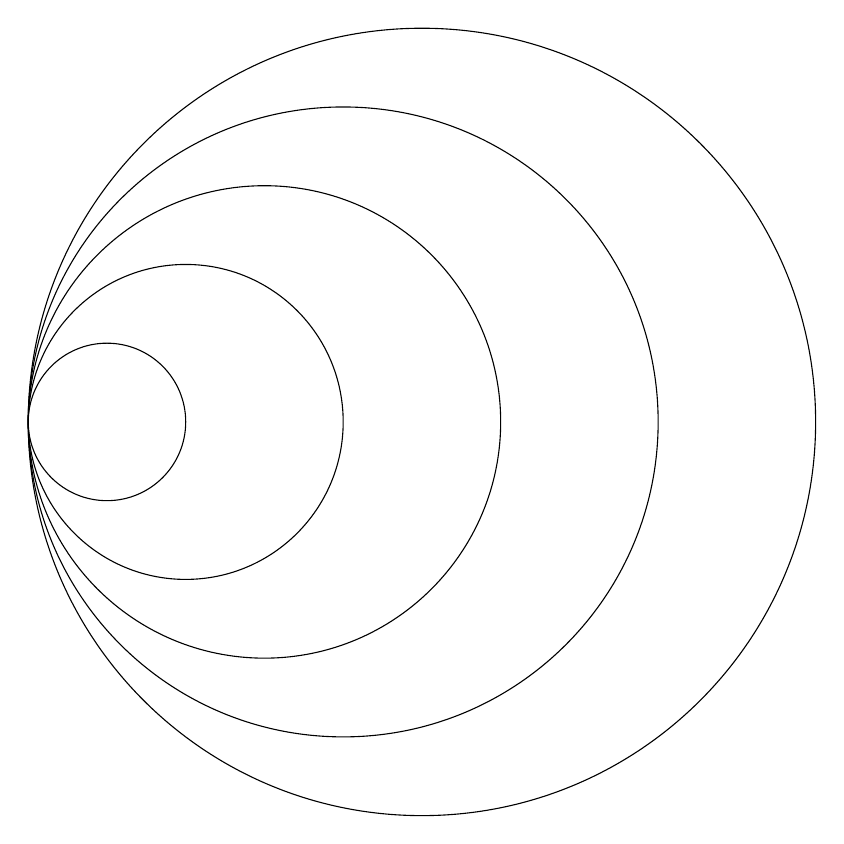
\begin{tikzpicture}
	\foreach \x in {1, ..., 5}
		\draw (\x, 0) circle (\x);
    \end{tikzpicture}

    \definecolor{myBlue}{HTML}{92ec93}
    \begin{tikzpicture}
	\foreach \x in {1, ..., 5}
		\shade[ball color=black!\x 0!myBlue] (\x, 0) circle (3mm);
    \end{tikzpicture}

    
\begin{tikzpicture}
	\foreach \x/\color in {1/green, 2/red, 3/blue, 4/yellow, 5/orange}
		\shade[ball color=\color] (\x, 0) circle (3mm);
    \end{tikzpicture}
\end{comment}

    % http://www.texample.net/tikz/examples/neural-network/
    \begin{tikzpicture}[shorten >=1pt,->,draw=black!50, node distance=\layersep]
	\tikzstyle{every pin edge}=[<-,shorten <=1pt]
	\tikzstyle{neuron}=[circle,fill=black!25,minimum size=17pt,inner sep=0pt]
	\tikzstyle{input neuron}=[neuron, fill=green!50];
	\tikzstyle{output neuron}=[neuron, fill=red!50];
	\tikzstyle{hidden neuron}=[neuron, fill=blue!50];
	\tikzstyle{annot} = [text width=4em, text centered]

	% Draw the input layer nodes
	\foreach \name / \y in {1, 2}
		\path[yshift=-0.5cm]
		node[input neuron, pin=left:Input \#\y] (I-\name) at (0,-\y) {};

	% Draw the hidden layer 1 nodes
	\foreach \name / \y in {1, ..., 4}
		\path[yshift=0.5cm]
		node[hidden neuron] (H1-\name) at (\layersep,-\y cm) {};

	% Draw the hidden layer 2 nodes
	\foreach \name / \y in {1, 2, 3}
		\node[hidden neuron] (H2-\name) at (2*\layersep,-\y cm) {};

	% Draw the output layer node
	\foreach \name/\y in {1, 2}
		%\node[output neuron,pin={[pin edge={->}]right:Output}, right of=H2-2] (O) {};
		\path[yshift=-0.5cm]
		node[output neuron, pin=right:Output \#\y] (O-\name) at (3*\layersep, -\y) {};

	% Connect every node in the input layer with every node in the
	% hidden layer.
	\foreach \source in {1, 2}
		\foreach \dest in {1, ..., 4}
			\path (I-\source) edge (H1-\dest);

	\foreach \source in {1, ..., 4}
		\foreach \dest in {1, 2, 3}
			\path (H1-\source) edge (H2-\dest);

	% Connect every node in the hidden layer with the output layer
	\foreach \source in {1, 2, 3}
		\foreach \dest in {1, 2}
			\path (H2-\source) edge (O-\dest);

	% Annotate the layers
	\node[annot,above of=H1-1, node distance=1cm] (hl1) {Hidden layer 1};
	\node[annot,left of=hl1] {Input layer};
	\node[annot,right of=hl1] (hl2) {Hidden layer 2};
	\node[annot,right of=hl2] {Output layer};
    \end{tikzpicture}

\end{document}

